\documentclass[journal,12pt,twocolumn]{IEEEtran}
\usepackage{setspace}
\usepackage{gensymb}
\usepackage{caption}
%\usepackage{multirow}
%\usepackage{multicolumn}
%\usepackage{subcaption}
%\doublespacing
\singlespacing
\usepackage{csvsimple}
\usepackage{amsmath}
\usepackage{multicol}
%\usepackage{enumerate}
\usepackage{amssymb}
%\usepackage{graphicx}
\usepackage{newfloat}
%\usepackage{syntax}
\usepackage{listings}
\usepackage{color}
\usepackage{tikz}
\usepackage{graphicx}
\usetikzlibrary{shapes,arrows}
\usepackage{chngcntr}
\counterwithin{figure}{section}
%\usepackage{graphicx}
%\usepackage{amssymb}
%\usepackage{relsize}
%\usepackage[cmex10]{amsmath}
%\usepackage{mathtools}
%\usepackage{amsthm}
%\interdisplaylinepenalty=2500
%\savesymbol{iint}
%\usepackage{txfonts}
%\restoresymbol{TXF}{iint}
%\usepackage{wasysym}
\usepackage{amsthm}
\usepackage{mathrsfs}
\usepackage{txfonts}
\usepackage{stfloats}
\usepackage{cite}
\usepackage{cases}
\usepackage{mathtools}
\usepackage{caption}
\usepackage{enumerate}	
\usepackage{enumitem}
\usepackage{amsmath}
%\usepackage{xtab}
\usepackage{longtable}
\usepackage{multirow}
%\usepackage{algorithm}
%\usepackage{algpseudocode}
\usepackage{enumitem}
\usepackage{mathtools}
\usepackage{hyperref}
%\usepackage[framemethod=tikz]{mdframed}
\usepackage{listings}
    %\usepackage[latin1]{inputenc}                                 %%
    \usepackage{color}                                            %%
    \usepackage{array}                                            %%
    \usepackage{longtable}                                        %%
    \usepackage{calc}                                             %%
    \usepackage{multirow}                                         %%
    \usepackage{hhline}                                           %%
    \usepackage{ifthen}                                           %%
  %optionally (for landscape tables embedded in another document): %%
    \usepackage{lscape}     


\usepackage{url}
\def\UrlBreaks{\do\/\do-}


%\usepackage{stmaryrd}


%\usepackage{wasysym}
%\newcounter{MYtempeqncnt}
\DeclareMathOperator*{\Res}{Res}
%\renewcommand{\baselinestretch}{2}
\renewcommand\thesection{\arabic{section}}
\renewcommand\thesubsection{\thesection.\arabic{subsection}}
\renewcommand\thesubsubsection{\thesubsection.\arabic{subsubsection}}

\renewcommand\thesectiondis{\arabic{section}}
\renewcommand\thesubsectiondis{\thesectiondis.\arabic{subsection}}
\renewcommand\thesubsubsectiondis{\thesubsectiondis.\arabic{subsubsection}}

% correct bad hyphenation here
\hyphenation{op-tical net-works semi-conduc-tor}

%\lstset{
%language=C,
%frame=single, 
%breaklines=true
%}

%\lstset{
	%%basicstyle=\small\ttfamily\bfseries,
	%%numberstyle=\small\ttfamily,
	%language=Octave,
	%backgroundcolor=\color{white},
	%%frame=single,
	%%keywordstyle=\bfseries,
	%%breaklines=true,
	%%showstringspaces=false,
	%%xleftmargin=-10mm,
	%%aboveskip=-1mm,
	%%belowskip=0mm
%}

%\surroundwithmdframed[width=\columnwidth]{lstlisting}
\def\inputGnumericTable{}                                 %%
\lstset{
%language=C,
frame=single, 
breaklines=true,
columns=fullflexible
}

\begin{document}
%
\tikzstyle{block} = [rectangle, draw,
    text width=3em, text centered, minimum height=3em]
\tikzstyle{sum} = [draw, circle, node distance=3cm]
\tikzstyle{input} = [coordinate]
\tikzstyle{output} = [coordinate]
\tikzstyle{pinstyle} = [pin edge={to-,thin,black}]

\theoremstyle{definition}
\newtheorem{theorem}{Theorem}[section]
\newtheorem{problem}{Problem}
\newtheorem{proposition}{Proposition}[section]
\newtheorem{lemma}{Lemma}[section]
\newtheorem{corollary}[theorem]{Corollary}
\newtheorem{example}{Example}[section]
\newtheorem{definition}{Definition}[section]
%\newtheorem{algorithm}{Algorithm}[section]
%\newtheorem{cor}{Corollary}
\newcommand{\BEQA}{\begin{eqnarray}}
\newcommand{\EEQA}{\end{eqnarray}}
\newcommand{\define}{\stackrel{\triangle}{=}}

\bibliographystyle{IEEEtran}
%\bibliographystyle{ieeetr}

\providecommand{\nCr}[2]{\,^{#1}C_{#2}} % nCr
\providecommand{\nPr}[2]{\,^{#1}P_{#2}} % nPr
\providecommand{\mbf}{\mathbf}
\providecommand{\pr}[1]{\ensuremath{\Pr\left(#1\right)}}
\providecommand{\qfunc}[1]{\ensuremath{Q\left(#1\right)}}
\providecommand{\sbrak}[1]{\ensuremath{{}\left[#1\right]}}
\providecommand{\lsbrak}[1]{\ensuremath{{}\left[#1\right.}}
\providecommand{\rsbrak}[1]{\ensuremath{{}\left.#1\right]}}
\providecommand{\brak}[1]{\ensuremath{\left(#1\right)}}
\providecommand{\lbrak}[1]{\ensuremath{\left(#1\right.}}
\providecommand{\rbrak}[1]{\ensuremath{\left.#1\right)}}
\providecommand{\cbrak}[1]{\ensuremath{\left\{#1\right\}}}
\providecommand{\lcbrak}[1]{\ensuremath{\left\{#1\right.}}
\providecommand{\rcbrak}[1]{\ensuremath{\left.#1\right\}}}
\theoremstyle{remark}
\newtheorem{rem}{Remark}
\newcommand{\sgn}{\mathop{\mathrm{sgn}}}
\providecommand{\pd}[2]{\ensuremath{\frac{\partial #1}{\partial #2}}}
\providecommand{\abs}[1]{\left\vert#1\right\vert}
\providecommand{\res}[1]{\Res\displaylimits_{#1}} 
\providecommand{\norm}[1]{\left\Vert#1\right\Vert}
\providecommand{\mtx}[1]{\mathbf{#1}}
\providecommand{\mean}[1]{E\left[ #1 \right]}
\providecommand{\fourier}{\overset{\mathcal{F}}{ \rightleftharpoons}}
\providecommand{\gauss}[2]{\ensuremath{\mathcal{N}(#1, #2)}}
%\providecommand{\hilbert}{\overset{\mathcal{H}}{ \rightleftharpoons}}
\providecommand{\system}{\overset{\mathcal{H}}{ \longleftrightarrow}}
	%\newcommand{\solution}[2]{\textbf{Solution:}{#1}}
\newcommand{\solution}{\noindent \textbf{Solution: }}
\newcommand{\myvec}[1]{\ensuremath{\begin{pmatrix}#1\end{pmatrix}}}
\providecommand{\dec}[2]{\ensuremath{\overset{#1}{\underset{#2}{\gtrless}}}}
\DeclarePairedDelimiter{\ceil}{\lceil}{\rceil}
%\numberwithin{equation}{section}
%\numberwithin{problem}{subsection}
%\numberwithin{definition}{subsection}
\makeatletter
\@addtoreset{figure}{section}
\makeatother

%\let\StandardTheFigure\thefigure
%\renewcommand{\thefigure}{\theproblem.\arabic{figure}}
\renewcommand{\thefigure}{\arabic{section}.\arabic{figure}}

%\numberwithin{figure}{subsection}

%\numberwithin{equation}{subsection}
%\numberwithin{equation}{section}
%\numberwithin{equation}{problem}
%\numberwithin{problem}{subsection}
%\numberwithin{problem}{section}
%%\numberwithin{definition}{subsection}
%\makeatletter
%\makeatother
%\makeatletter
%\@addtoreset{figure}{section}
%\@addtoreset{table}{section}
%\makeatother

\let\StandardTheFigure\thefigure
\let\StandardTheTable\thetable
\let\vec\mathbf
\numberwithin{equation}{section}

\vspace{3cm}


\title{%Convex Optimization in Python
	Random Numbers
}
%\title{
%	\logo{Matrix Analysis through Octave}{\begin{center}\includegraphics[scale=.24]{tlc}\end{center}}{}{HAMDSP}
%}

% paper title
% can use linebreaks \\ within to get better formatting as desired
%\title{Matrix Analysis through Octave}
%
%
% author names and IEEE memberships
% note positions of commas and nonbreaking spaces ( ~ ) LaTeX will not break
% a structure at a ~ so this keeps an author's name from being broken across
% two lines.
% use \thanks{} to gain access to the first footnote area
% a separate \thanks must be used for each paragraph as LaTeX2e's \thanks
% was not built to handle multiple paragraphs
%

\author{Gautam Singh}
\maketitle

\tableofcontents

\bigskip

%\renewcommand{\thefigure}{\theenumi}
%\renewcommand{\thetable}{\theenumi}

\begin{abstract}
	This manual provides a simple introduction to the generation of random numbers. Commands that must be executed in a *NIX shell are preceded by a \$ symbol.
\end{abstract}
%%
\section{Uniform Random Numbers}
Let $U$ be a uniform random variable between 0 and 1.
\begin{enumerate}[label=\thesection.\arabic*
,ref=\thesection.\theenumi]
\item Generate $10^6$ samples of $U$ using a C program and save into a file called uni.dat .

\solution Download the following files
\begin{lstlisting}
$ wget https://raw.githubusercontent.com/goats-9/ai1110-assignments/master/manual/codes/1_1.c
$ wget https://raw.githubusercontent.com/goats-9/ai1110-assignments/master/manual/codes/1_1.h
\end{lstlisting}
and compile and execute the C program using
\begin{lstlisting}
$ gcc 1_1.c -lm -Wall -g
$ ./a.out
\end{lstlisting}

%
\item
Load the uni.dat file into python and plot the empirical CDF of $U$ using the samples in uni.dat. The CDF is defined as
\begin{align}
F_{U}(x) = \pr{U \leq x}
\end{align}

\solution  The following code plots Fig. \ref{fig:uni_cdf}
\begin{lstlisting}
$ wget https://raw.githubusercontent.com/goats-9/ai1110-assignments/master/manual/codes/1_2.py
\end{lstlisting}
It is executed with
\begin{lstlisting}
$ python3 1_2.py
\end{lstlisting}
\begin{figure}
\centering
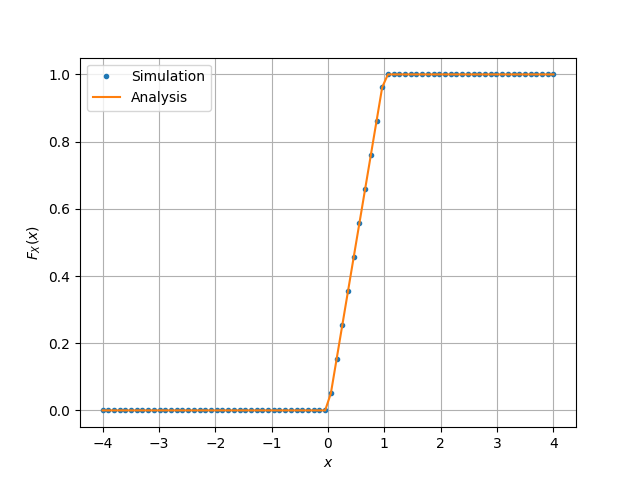
\includegraphics[width=\columnwidth]{./figs/1_2.png}
\caption{The CDF of $U$}
\label{fig:uni_cdf}
\end{figure}

%
\item
Find a theoretical expression for $F_{U}(x)$.

\solution
The CDF of $U$ is given by
		\begin{align}
			F_U(x) = \pr{U \leq x} = \int_{-\infty}^{x}p_U(u)du
		\end{align}
We now have three cases:
		\begin{enumerate}
			\item $x < 0$: $p_X(x) = 0$, and hence $F_U(x) = 0$.
			\item $0 \leq x < 1$: Here,
				\begin{align}
					F_U(x) = \int_{0}^{x}du = x
					\label{eq:cdf-uni}
				\end{align}
			\item $x \geq 1$: Put $x = 1$ in \eqref{eq:cdf-uni} as $U$ is uniform in [0, 1] to get $F_U(x) = 1$.
		\end{enumerate}
Therefore,
		\begin{align}
			F_U(x) = 
			\begin{cases}
				0 & x < 0 \\
				x & 0 \leq x < 1 \\
				1 & x \geq 1
			\end{cases}
			\label{eq:cdf-ans}
		\end{align}
This is verified in Figure \eqref{fig:uni_cdf}
\item
The mean of $U$ is defined as
%
\begin{equation}
E\sbrak{U} = \frac{1}{N}\sum_{i=1}^{N}U_i
	\label{eq:mean-form}
\end{equation}
%
and its variance as
%
\begin{equation}
\text{var}\sbrak{U} = E\sbrak{U- E\sbrak{U}}^2 
	\label{eq:var-form}
\end{equation}

Write a C program to  find the mean and variance of $U$.

\solution
The C program can be downloaded using
\begin{lstlisting}
$ wget https://raw.githubusercontent.com/goats-9/ai1110-assignments/master/manual/codes/1_4.c
\end{lstlisting}
and compiled and executed with
\begin{lstlisting}
$ gcc 1_4.c -lm -Wall -g
$ ./a.out
\end{lstlisting}
The calculated mean is 0.500007 and the calculated variance is 0.083301.

\item Verify your result theoretically given that
\end{enumerate}
%
\begin{equation}
E\sbrak{U^k} = \int_{-\infty}^{\infty}x^kdF_{U}(x)dx
\end{equation}
\solution
We write
\begin{align}
	E\sbrak{U^2} &= \int_{-\infty}^{\infty}x^2dF_U(x) \\
	&= \int_{-\infty}^{\infty}x^2p_U(x)dx \\
	&= \int_{0}^{1}x^2dx = \frac{1}{3}
\end{align}
and
\begin{align}
	E\sbrak{U} &= \int_{-\infty}^{\infty}xdF_U(x) \\
	&= \int_{-\infty}^{\infty}xp_U(x)dx \\
	&= \int_{0}^{1}xdx = \frac{1}{2}
\end{align}
which checks out with the empirical mean on 0.500007. Now, using linearity of expectation,
\begin{align}
	\text{var}\sbrak{U} &= E\sbrak{U - E\sbrak{U}}^2 \\
	&= E\sbrak{U^2 - 2UE\sbrak{U} + \left(E\sbrak{U}\right)^2} \\
	&= E\sbrak{U^2} - 2\left(E\sbrak{U}\right)^2 + \left(E\sbrak{U}\right)^2 \\
	&= E\sbrak{U^2} - \left(E\sbrak{U}\right)^2 = \frac{1}{3} - \frac{1}{4} = \frac{1}{12}
\end{align}
and this checks out with the empirical variance 0.083301 of the sample data.
\section{Central Limit Theorem}
%
\begin{enumerate}[label=\thesection.\arabic*
,ref=\thesection.\theenumi]

%
\item
Generate $10^6$ samples of the random variable
%
\begin{equation}
X = \sum_{i=1}^{12}U_i -6
\end{equation}
%
using a C program, where $U_i, i = 1,2,\dots, 12$ are  a set of independent uniform random variables between 0 and 1
and save in a file called gau.dat

\solution
The sample data is generated by the C file in Question 1.1.
%
\item
Load gau.dat in python and plot the empirical CDF of $X$ using the samples in gau.dat. What properties does a CDF have?

\solution The CDF of $X$ is plotted in Fig. \ref{fig:gauss_cdf}
\begin{figure}[!htb]
\centering
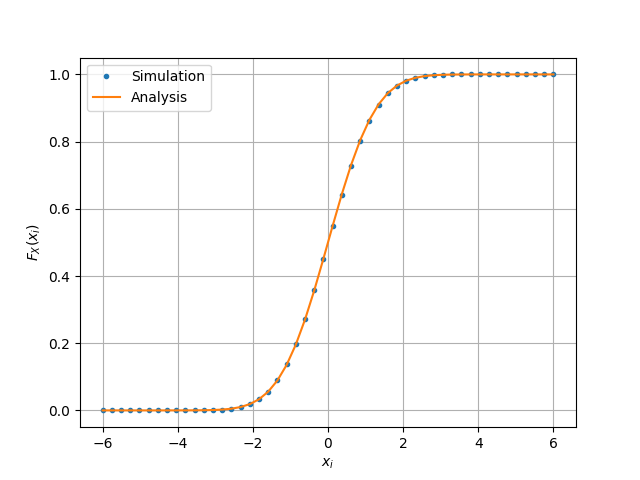
\includegraphics[width=\columnwidth]{./figs/2_2.png}
\caption{The CDF of $X$}
\label{fig:gauss_cdf}
\end{figure}
Download the Python code using
\begin{lstlisting}
$ wget https://raw.githubusercontent.com/goats-9/ai1110-assignments/master/manual/codes/2_2.py
\end{lstlisting}
and execute it with
\begin{lstlisting}
$ python3 2_2.py
\end{lstlisting}
The CDF of a probability distribution has the following properties:
		\begin{enumerate}
			\item It is non-decreasing
			\item It is right-continuous
			\item $\lim_{x \to -\infty}F_X(x) = 0$
			\item $\lim_{x \to \infty}F_X(x) = 1$
		\end{enumerate}
The CDF of the normal distribution is expressed in terms of the Q-function as $F_X(x) = 1 - Q(x)$.
\item
Load gau.dat in python and plot the empirical PDF of $X$ using the samples in gau.dat. The PDF of $X$ is defined as
\begin{align}
p_{X}(x) = \frac{d}{dx}F_{X}(x)
	\label{eq:pdf-cdf}
\end{align}
What properties does the PDF have?

\solution The PDF of $X$ is plotted in Fig. \ref{fig:gauss_pdf} using the code below
\begin{lstlisting}
$ wget https://raw.githubusercontent.com/goats-9/ai1110-assignments/master/manual/codes/2_3.py
\end{lstlisting}
The figure is generated using
\begin{lstlisting}
$ python3 2_3.py
\end{lstlisting}
The properties of a PDF are as follows:
		\begin{enumerate}
			\item $\forall x \in \mathbb{R}$, $p_X(x) \geq 0$
			\item $\int_{-\infty}^{\infty}p_X(x)dx = 1$
			\item For $a < b$, $a, b \in \mathbb{R}$ 
				\begin{align}
					\pr{a < X < b} &= \pr{a \leq X \leq b} \\
					&= \int_{a}^{b}p_X(x)dx
				\end{align}
				If we take $a = b$, then we get $\pr{X = a} = 0$.
		\end{enumerate}
\begin{figure}
\centering
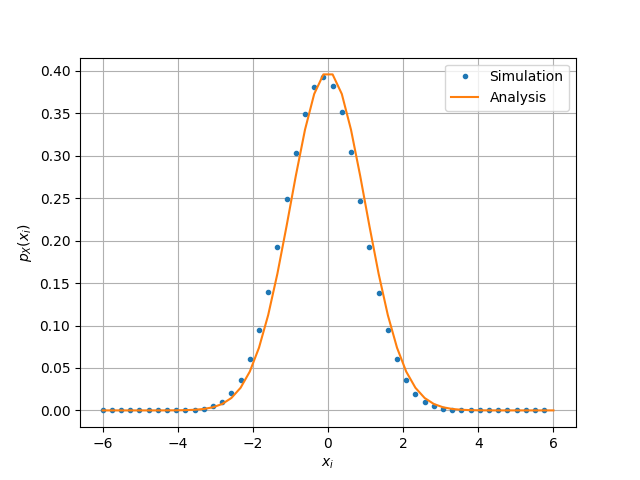
\includegraphics[width=\columnwidth]{./figs/2_3.png}
\caption{The PDF of $X$}
\label{fig:gauss_pdf}
\end{figure}

\item Find the mean and variance of $X$ by writing a C program.

\solution
The mean and variance have been calculated using \eqref{eq:mean-form} and \eqref{eq:var-form} respectively.

\noindent The C program can be downloaded using
\begin{lstlisting}
$ wget https://raw.githubusercontent.com/goats-9/ai1110-assignments/master/manual/codes/2_4.c
\end{lstlisting}
and compiled and executed with the following commands
\begin{lstlisting}
$ gcc 2_4.c -lm -Wall -g
$ ./a.out
\end{lstlisting}
The calculated mean is 0.000326 and the calculated variance is 1.000906.

\item Given that 
\begin{align}
p_{X}(x) = \frac{1}{\sqrt{2\pi}}\exp\brak{-\frac{x^2}{2}}, -\infty < x < \infty,
\end{align}
repeat the above exercise theoretically.

\solution
The mean is given by
		\begin{align}
			E\sbrak{X} = \int_{-\infty}^{\infty}x\frac{1}{\sqrt{2\pi}}\exp{\left(-\frac{x^2}{2}\right)} = 0
			\label{eq:gau-mean}
		\end{align}
as the integrand is odd. This checks out with the empirical mean of 0.000326. The variance is given by
		\begin{align}
			\text{var}\sbrak{X} &= E\sbrak{X^2} - \left(E\sbrak{X}\right)^2 \\
			&= \int_{-\infty}^{\infty}x^2\frac{1}{\sqrt{2\pi}}\exp{\left(-\frac{x^2}{2}\right)}dx \label{eq:int} \\
			&= \int_{0}^{\infty}\frac{2}{\sqrt{2\pi}}\sqrt{2t}e^{-t}dt \\
			&= \frac{2}{\sqrt{\pi}}\Gamma\left(\frac{3}{2}\right) \\
			&= \frac{1}{\sqrt{\pi}}\Gamma\left(\frac{1}{2}\right) = 1
			\label{eq:gau-var}
		\end{align}
where we have used $t = \frac{x^2}{2}$ and so $dt = xdx$. We have also used the gamma function defined as
\begin{align}
	\Gamma(n) &= \int_{-\infty}^{\infty}x^{n - 1}e^{-x}dx \\
	\Gamma(n) &= (n - 1)\Gamma(n - 1)\ \text{for $n > 1$}
\end{align}
and the fact that $\Gamma(1/2) = \sqrt{\pi}$.
This agrees with the empirical variance of 1.000906.
%
\end{enumerate}
\section{From Uniform to Other}
\begin{enumerate}[label=\thesection.\arabic*
,ref=\thesection.\theenumi]
%
\item
Generate samples of 
%
\begin{equation}
V = -2\ln\brak{1-U}
\end{equation}
%
and plot its CDF. 

\solution
The relevant python code is at
\begin{lstlisting}
$ wget https://raw.githubusercontent.com/goats-9/ai1110-assignments/master/manual/codes/3_1.py
\end{lstlisting}
and can be executed with
\begin{lstlisting}
$ python3 3_1.py
\end{lstlisting}
The CDF is plotted in Figure \eqref{fig:exp_cdf}.
\begin{figure}[!htb] 
\centering
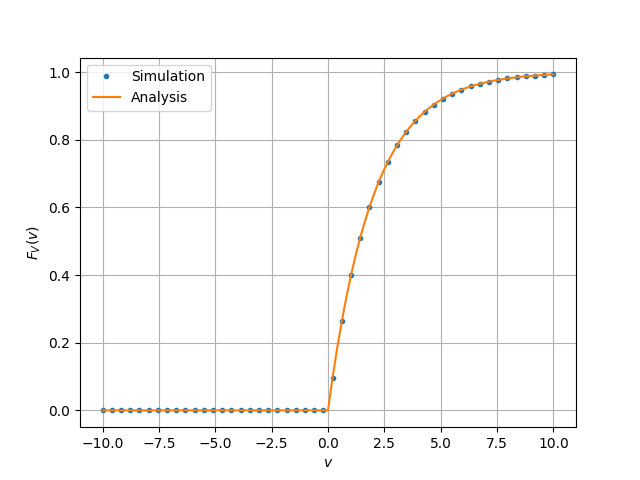
\includegraphics[width=\columnwidth]{./figs/3_1.png}
\caption{The CDF of $V$}
\label{fig:exp_cdf}
\end{figure}

\item Find a theoretical expression for $F_V(x)$.

\solution
Note that the function 
		\begin{align}
			v = f(u) = -2\ln{(1 - u)}
		\end{align}
is monotonically increasing in [0, 1] and $v \in \mathbb{R^+}$. Hence, it is invertible and the inverse function is given by
		\begin{align}
			u = f^{-1}(v) = 1 - \exp{\left(-\frac{v}{2}\right)}
		\end{align}
		Therefore, from the monotonicity of $v$, and using \eqref{eq:cdf-ans},
		\begin{align}
			F_V(v) &= F_U\left(1 - \exp{\left(-\frac{v}{2}\right)}\right) \\
			\implies F_V(v) &= 
			\begin{cases}
				0 & v < 0 \\
				1 - \exp{\left(-\frac{v}{2}\right)} & v \geq 0
			\end{cases}
			\label{eq:f-v}
		\end{align}
%
%\item
%Generate the Rayleigh distribution from Uniform. Verify your result through graphical plots.
\end{enumerate}

\section{Triangular Distribution}
\begin{enumerate}[label=\thesection.\arabic*
,ref=\thesection.\theenumi]
\item Generate
	\begin{align}
		T = U_1 + U_2
	\end{align}

\solution
The samples are generated in the C file exrand.c in 1.1 as the file tri.dat.

\item Find the CDF of $T$.

\solution
The Python code for the figure is at
\begin{lstlisting}
$ wget https://raw.githubusercontent.com/goats-9/ai1110-assignments/master/manual/codes/4_2.py
\end{lstlisting}
and can be run using
\begin{lstlisting}
$ python3 4_2.py
\end{lstlisting}
\begin{figure}[!htb]
	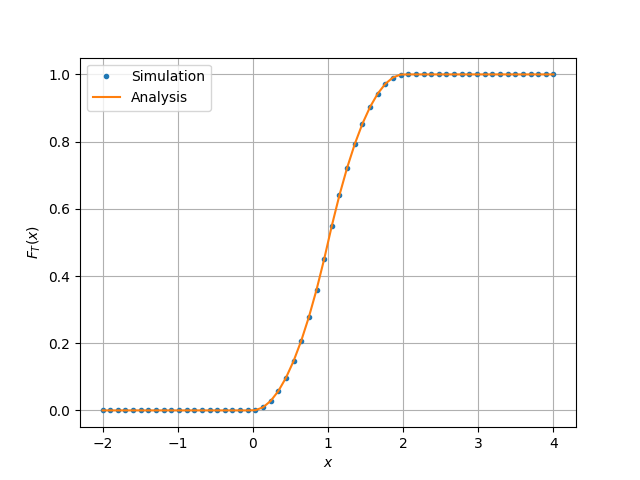
\includegraphics[width=\columnwidth]{figs/4_2.png}
	\caption{The CDF of $T$}
	\label{fig:tri-cdf}
\end{figure}
\item Find the PDF of $T$.
	\begin{figure}
		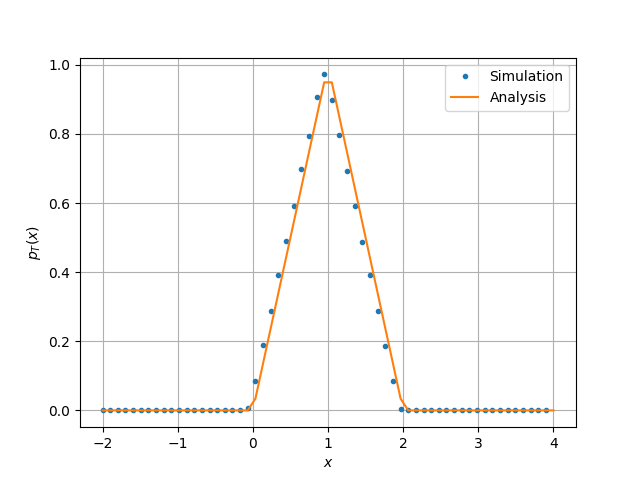
\includegraphics[width=\columnwidth]{figs/4_3.png}
		\caption{The PDF of $T$}
		\label{fig:tri-pdf}
	\end{figure}

\solution
The Python code for the figure can be downloaded using 
\begin{lstlisting}
$ wget https://raw.githubusercontent.com/goats-9/ai1110-assignments/master/manual/codes/4_3.py
\end{lstlisting}
and run using
\begin{lstlisting}
$ python3 4_3.py
\end{lstlisting}

\item Find the theoretical PDF and CDF of $T$.

\solution
We write,
		\begin{align}
			F_T(t) &= \pr{U_1 + U_2 \leq t} \\
			&= \pr{U_1 \leq t - U_2} \\
			&= \int_{0}^{1}F_{U_1}(t - x)p_{U_2}(x)dx
		\end{align}
		where $U_1$ and $U_2$ are uniform i.i.d. random variables in [0, 1]. Then, $0 \leq U_1 + U_2 \leq 2$.
We have three cases:
		\begin{enumerate}
			\item $t < 0$: Using \autoref{eq:cdf-ans}, $F_T(t) = 0$.
			\item $0 \leq t < 1$: We have,
				\begin{align}
					F_T(t) = \int_{0}^{t}(t - x)dx = \frac{t^2}{2}
				\end{align}
			\item $1 \leq t < 2$: Here, we get
				\begin{align}
					F_T(t) &= \int_{0}^{t - 1}dx + \int_{t - 1}^{1}(t - x)dx \\
					&= t - 1 + t(2 - t) - \frac{1 - (t - 1)^2}{2} \\
					&= -\frac{t^2}{2} + 2t - 1
				\end{align}
			\item $t \geq 2$: Here, $F_T(t) = 1$.
		\end{enumerate}
Therefore,
		\begin{align}
			F_T(t) = 
			\begin{cases} 
				0 & t < 0 \\
				\frac{t^2}{2} &  0 \leq t < 1 \\
				-\frac{t^2}{2} + 2t - 1 & 1 \leq t < 2 \\
				1 & t \geq 2
			\end{cases}
			\label{eq:cdf-tri}
		\end{align}
Using \autoref{eq:pdf-cdf}, 
		\begin{align}
			p_T(t) = 
			\begin{cases}
				t & 0 \leq t < 1 \\
				2 - t & 1 \leq t < 2 \\
				0 & \text{otherwise}
			\end{cases}
			\label{eq:pdf-tri}
		\end{align}

\item Verify your results through a plot.

\solution
This has been done in the plots \eqref{fig:tri-cdf} and \eqref{fig:tri-pdf}.
\end{enumerate}

\section{Maximum Likelihood}
\begin{enumerate}[label=\thesection.\arabic*
,ref=\thesection.\theenumi]
\item Generate equiprobable $X \in \cbrak{1, -1}$.

\solution
The C file in Question 1.1 generates samples of $X$ in the file data/ber.dat.

\item Generate 
	\begin{align}
		Y = AX + N
	\end{align}
where $A  = 5 \text{ dB}, X \in \cbrak{1, -1}$ is Bernoulli and $N \sim \gauss{0}{1}$.

\solution
The C file in Question 1.1 generates the numbers in the file data/gau\_ber.dat
\item Plot Y using a scatter plot.

\solution
The Python code can be downloaded using
\begin{lstlisting}
$ wget https://raw.githubusercontent.com/goats-9/ai1110-assignments/master/manual/codes/5_2.py
\end{lstlisting}
and run using
\begin{lstlisting}
$ python3 5_2.py
\end{lstlisting}
\begin{figure}[!htb]
	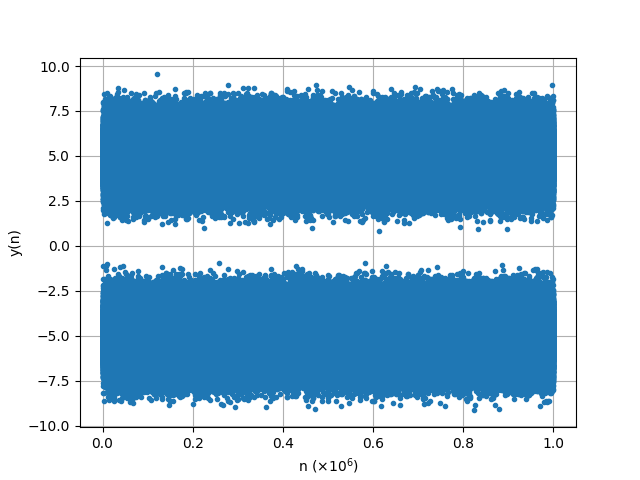
\includegraphics[width=\columnwidth]{figs/5_2.png}
	\caption{Plot of $Y$}
	\label{fig:wave}
\end{figure}

\item Guess how to estimate $X$ from $Y$.

\solution
From the plot of $Y$, we see that the estimate model can be written as
\begin{align}
	\hat{X} = 
	\begin{cases}
		1 & Y > 0 \\
		0 & Y < 0
	\end{cases}
\end{align}

\item Find 
	\begin{align}
		P_{e|0} = \pr{\hat{X} = -1|X = 1}
	\end{align}
and
	\begin{align}
		P_{e|1} = \pr{\hat{X} = 1|X = -1}
	\end{align}

\solution
Letting $X = 1$ and $X = -1$ respectively, we see the number of mismatched data points to compute the error probabilities. The simulation is coded in
\begin{lstlisting}
$ wget https://raw.githubusercontent.com/goats-9/ai1110-assignments/master/manual/codes/5_4.py
\end{lstlisting}
and can be run by typing
\begin{lstlisting}
$ python3 5_4.py
\end{lstlisting}
The results are
		\begin{align}
			P_{e|0} = 5.33 \times 10^{-4} \\
			P_{e|1} = 5.57 \times 10^{-4}
		\end{align}
\item Find $P_e$ assuming that $X$ has equiprobable symbols.

\solution
Here, $\pr{X = 1} = \pr{X = -1} = 0.5$. Thus,
	\begin{align}
		P_e &= \pr{X = 1}P_{e|1} + \pr{X = -1}P_{e|0} \label{eq:pe-gen} \\
		&= \frac{1}{2}\brak{P_{e|0} + P_{e|1}} = 5.45 \times 10^{-4}
	\end{align}
\item Verify by plotting the theoretical $P_e$ wrt $A$ from 0 dB to 10 dB.

\solution
We note that 
\begin{align}
	P_{e|0} &= \pr{\hat{X} = 1 | X = -1}\\
	&= \pr{Y > 0 | X = -1} \\
	&= \pr{AX + N > 0 | X = -1} \label{eq:thresh} \\
	&= \pr{N > A | X = -1} = \qfunc{A}
\end{align}
since $X$ and $N$ are independent. Writing a similar expression for $P_{e|1}$ and noting that 
\begin{align}
	\pr{N < -A} = \pr{N > A} = \qfunc{A}
\end{align}
it follows that $P_e = \qfunc{A}$. This is the idea used to plot the theoretical $P_e$. The plot is coded both in the rectangular axes and the semilog-y axes. Download the relevant codes using 
\begin{lstlisting}
$ wget https://raw.githubusercontent.com/goats-9/ai1110-assignments/master/manual/codes/5_6.py
$ wget https://raw.githubusercontent.com/goats-9/ai1110-assignments/master/manual/codes/5_6_semilog.py
\end{lstlisting}
and execute them using
\begin{lstlisting}
$ python3 5_6.py
$ python3 5_6_semilogy.py
\end{lstlisting}

\begin{figure}[!htb]
	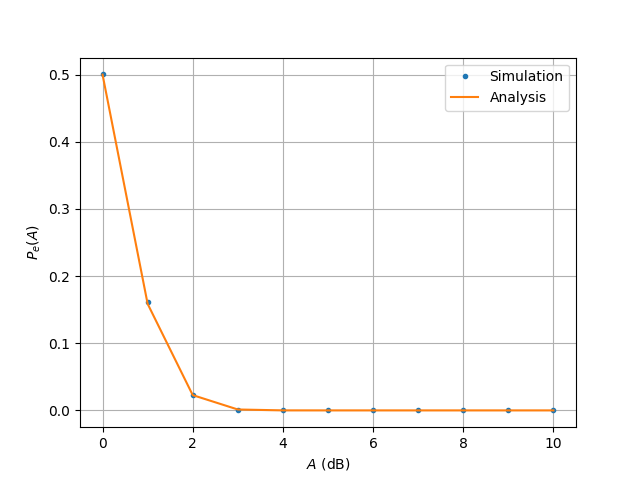
\includegraphics[width=\columnwidth]{figs/5_6.png}
	\caption{$P_e(A)$ (rectangular axes)}
	\label{fig:ber-snr}
\end{figure}
\begin{figure}[!htb]
	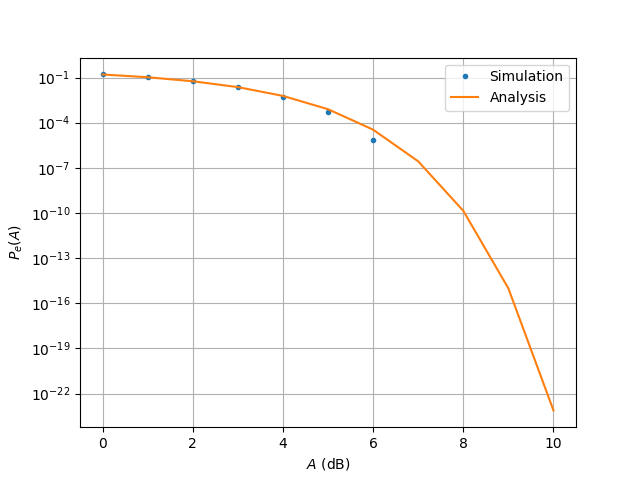
\includegraphics[width=\columnwidth]{figs/5_6_semilogy.png}
	\caption{$P_e(A)$ (semilog-y axes)}
	\label{fig:ber-snr-semilog}
\end{figure}
\item Now, consider a threshold $\delta$ while estimating $X$ from $Y$. Find the value of $\delta$ that maximizes the theoretical $P_e$.

\solution
Replacing the $0$ in \eqref{eq:thresh} with $\delta$ and performing a similar operation for $P_{e|1}$, we get
\begin{align}
	P_e &= \pr{X = -1}\qfunc{A + \delta} \nonumber \\ 
	&+ \pr{X = 1}\qfunc{A - \delta} \label{eq:delta-gen} \\
	&= \frac{1}{2}\brak{\qfunc{A + \delta} + \qfunc{A - \delta}} 
	\label{eq:func-delta}
\end{align}
Differentiating with respect to $\delta$ leads to the equation (here $f_N$ denotes standard normal distibution)
\begin{align}
	f_N\brak{A + \delta} = f_N\brak{A - \delta}
\end{align}
which implies that for $A \neq 0,\ \delta = 0$ and for $A = 0,\ \delta \in \mathbb{R}$. 

\item Repeat the above exercise when 
	\begin{align}
		p_X(1) = p
	\end{align}

\solution Using \eqref{eq:delta-gen} and following a similar procedure as in the previous question, we see that
\begin{align}
	pf_N\brak{A - \delta} &= \brak{1 - p}f_N\brak{A + \delta} \\
	pe^{-\frac{\brak{A - \delta}^2}{2}} &= \brak{1 - p}e^{-\frac{\brak{A + \delta}^2}{2}} \\
	\implies \delta &= \frac{1}{2A}\ln{\brak{\frac{1 - p}{p}}}
	\label{eq:delta-sol}
\end{align}
\item Repeat the above exercise using MAP criterion.

\solution Using Bayes' Theorem, we get
\begin{align}
	&\pr{X = 1 | Y = y} \nonumber \\
	&= \frac{\pr{N = y - A | X = 1}\pr{X = 1}}{p_Y\brak{y}} \\ 
	&= \frac{pf_N\brak{y - A}}{pf_N\brak{y - A} + \brak{1 - p}f_N\brak{y + A}} \\
	&= \frac{p}{p + \brak{1 - p}e^{-2yA}} 
\end{align}
and
\begin{align}
	&\pr{X = -1 | Y = y} \nonumber \\
	&= \frac{\pr{N = y + A | X = -1}\pr{X = -1}}{p_Y\brak{y}} \\ 
	&= \frac{\brak{1 - p}f_N\brak{y + A}}{pf_N\brak{y - A} + \brak{1 - p}f_N\brak{y + A}} \\
	&= \frac{1 - p}{\brak{1 - p} + pe^{2yA}} 
\end{align}
Hence, 
\begin{align}
	\frac{p}{p + \brak{1 - p}e^{-2yA}} &\gtrless \frac{1 - p}{\brak{1 - p} + pe^{2yA}} \\
	\implies p^2e^{2yA} &\gtrless \brak{1 - p}^2e^{-2yA} \\
	\implies y &\gtrless \frac{1}{2A}\ln{\brak{\frac{1 - p}{p}}}
\end{align}
\end{enumerate}

\section{Gaussian to Other}
\begin{enumerate}[label=\thesection.\arabic*
,ref=\thesection.\theenumi]
\item Let $X_1 \sim \gauss{0}{1}$ and $X_2 \sim \gauss{0}{1}$. Plot the CDF and PDF of
	\begin{align}
		V = X_1^2 + X_2^2
	\end{align}

\solution
We transform the variables $X_1$ and $X_2$ as:
		\begin{align}
			X_1 = R\cos{\Theta} \\
			X_2 = R\sin{\Theta}
		\end{align}
where $R \in [0, \infty), \Theta \in [0, 2\pi)$. The Jacobian Matrix for this transformation is given by
		\begin{align}
			\mtx{J} &= \myvec{\pd{X_1}{R} & \pd{X_2}{R} \\
							 \pd{X_1}{\Theta} & \pd{X_2}{\Theta}} \\
					&= \myvec{\cos{\Theta} & \sin{\Theta} \\
							  -R\sin{\Theta} & R\cos{\Theta}} \\
			\implies |\mtx{J}| &= R
			\label{eq:Jacobian}
		\end{align}
We also know that
		\begin{align}
			|\mtx{J}|p_{X_1, X_2}(x_1, x_2) &= p_{R, \Theta}(r, \theta) \\
			\implies p_{R, \Theta}(r, \theta) &= Rp_{X_1}(x_1)p_{X_2}(x_2) \label{eq:iid-split} \\
			&= \frac{R}{2\pi}\exp{\brak{-\frac{X_1^2 + X_2^2}{2}}} \\
			&= \frac{R}{2\pi}\exp{\brak{-\frac{R^2}{2}}}
			\label{eq:joint}
		\end{align}
where \eqref{eq:iid-split} follows as $X_1, X_2$ are iid random variables. Thus,
		\begin{align}
			p_R(r) &= \int_{0}^{2\pi}p_{R, \Theta}(r, \theta)d\theta \\
			&= R\exp{\brak{-\frac{R^2}{2}}}
		\end{align}
However, $V = X_1^2 + X_2^2 = R^2 \geq 0$, thus $F_V(x) = 0$ for $x < 0$ and
		\begin{align}
			F_V(x) &= F_R(\sqrt{x}) \\ 
			&= \int_{0}^{\sqrt{x}}r\exp{\brak{-\frac{r^2}{2}}}dr \\
			&= \int_{0}^{\frac{x}{2}}e^{-t}dt = 1 - e^{-\frac{x}{2}}
		\end{align}
where $t = \frac{r^2}{2}$ for $x \geq 0$, thus
		\begin{align}
			p_V(x) = \frac{1}{2}e^{-\frac{x}{2}}
		\end{align}
Hence, 
		\begin{align}
			F_V(x) = 
			\begin{cases}
				1 - e^{-\frac{x}{2}} & x \geq 0 \\
				0 & x < 0 
			\end{cases} \label{eq:chi-cdf} \\
			p_V(x) = 
			\begin{cases}
				\frac{1}{2}e^{-\frac{x}{2}} & x \geq 0 \\
				0 & x < 0
			\end{cases} \label{eq:chi-pdf} 
		\end{align}
The equations \eqref{eq:chi-cdf} and \eqref{eq:chi-pdf} have been used to generate the plots. The Python code can be downloaded from
\begin{lstlisting}
$ wget https://raw.githubusercontent.com/goats-9/ai1110-assignments/master/manual/codes/6_1_cdf.py
$ wget https://raw.githubusercontent.com/goats-9/ai1110-assignments/master/manual/codes/6_1_pdf.py
\end{lstlisting}
Execute the codes by typing the commands
\begin{lstlisting}
$ python3 6_1_cdf.py
$ python3 6_1_pdf.py
\end{lstlisting}
\begin{figure}[!htb]
	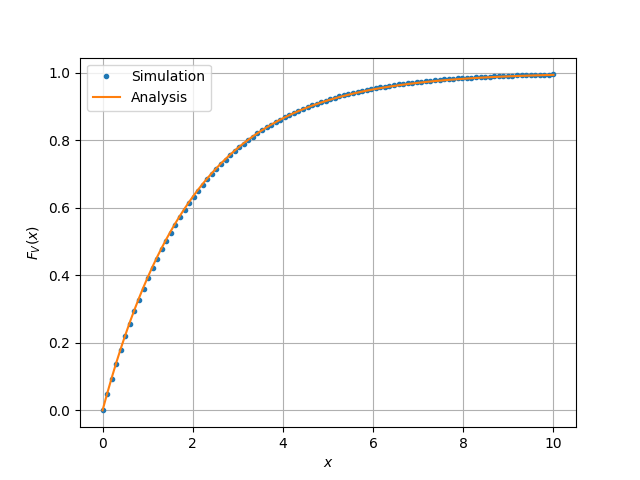
\includegraphics[width=\columnwidth]{figs/6_1_cdf.png}
	\caption{CDF of $V$}
	\label{fig:chi-cdf}
\end{figure}
\begin{figure}[!htb]	
	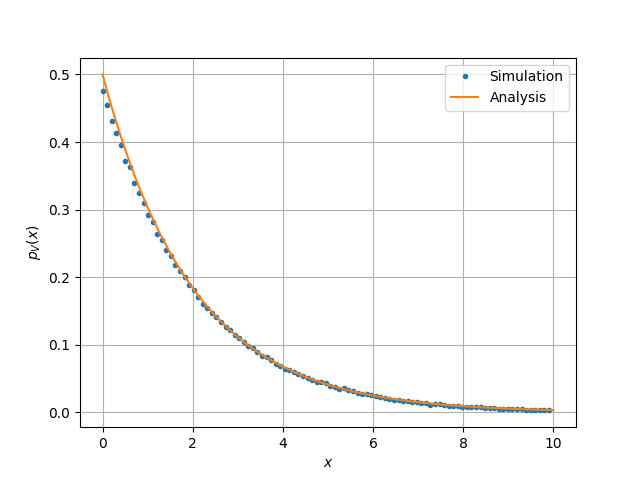
\includegraphics[width=\columnwidth]{figs/6_1_pdf.png}
	\caption{PDF of $V$}
	\label{fig:chi-pdf}
\end{figure}
\item If
	\begin{align}
		F_V(x) = 
		\begin{cases}
			1 - e^{-\alpha x} & x \geq 0 \\
			0 & x < 0
		\end{cases}
	\end{align}
find $\alpha$.

\solution
		From \eqref{eq:chi-cdf}, it is clear that $\alpha = 0.5$.

\item Plot the CDF and PDF of 
	\begin{align}
		A = \sqrt{V}
	\end{align}

\solution

Note that for $x \geq 0$,
\begin{align}
	F_A(x) &= \pr{A \leq x} \\
	&= \pr{\sqrt{V} \leq x} \\
	&= \pr{V \leq x^2} \\
	&= F_V(x^2) = 1 - e^{-\frac{x^2}{2}}
\end{align}
and so,
\begin{align}
	p_A(x) = xe^{-\frac{x^2}{2}}
\end{align}
Thus, the CDF and PDF of $A$ is given by
\begin{align}
	F_V(x) = 
	\begin{cases}
		1 - e^{-\frac{x^2}{2}} & x \geq 0 \\
		0 & x < 0 
	\end{cases} \label{eq:ral-cdf} \\
	p_V(x) = 
	\begin{cases}
		xe^{-\frac{x}{2}} & x \geq 0 \\
		0 & x < 0
	\end{cases} \label{eq:ral-pdf} 
\end{align}
The Python codes for the plots are at
\begin{lstlisting}
$ wget https://raw.githubusercontent.com/goats-9/ai1110-assignments/master/manual/codes/6_3_cdf.py
$ wget https://raw.githubusercontent.com/goats-9/ai1110-assignments/master/manual/codes/6_3_pdf.py
\end{lstlisting}
and can be executed using
\begin{lstlisting}
$ python3 6_3_cdf.py
$ python3 6_3_pdf.py
\end{lstlisting}
\begin{figure}[!htb]
	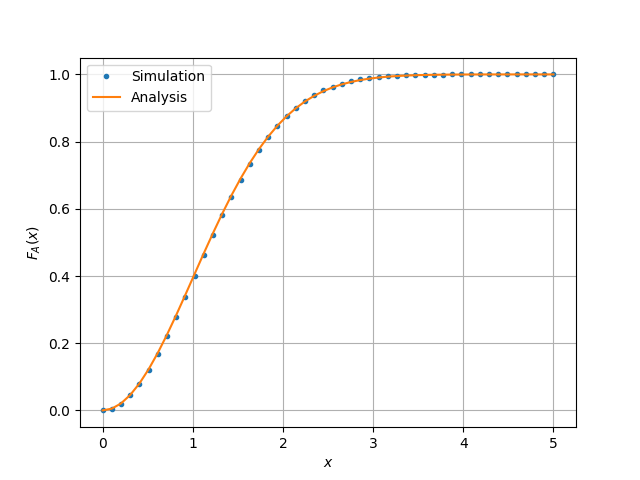
\includegraphics[width=\columnwidth]{figs/6_3_cdf.png}
	\caption{CDF of $A$}
	\label{fig:ral-cdf}
\end{figure}
\begin{figure}[!htb]
	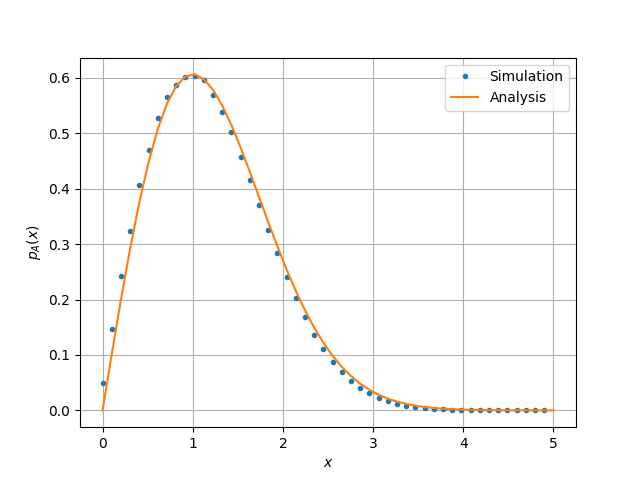
\includegraphics[width=\columnwidth]{figs/6_3_pdf.png}
	\caption{PDF of $A$}
	\label{fig:ral-pdf}
\end{figure}
\end{enumerate}

\section{Conditional Probability}
\begin{enumerate}[label=\thesection.\arabic*
,ref=\thesection.\theenumi]
\item Plot 
	\begin{align}
		P_e = \pr{\hat{X} = -1|X = 1}
	\end{align}
for 
	\begin{align}
		Y = AX + N
	\end{align}
where $A$ is Rayleigh with $E\sbrak{A^2} = \gamma,\ N \sim \gauss{0}{1},\ X \in \cbrak{1, -1}$ for $0 \leq \gamma \leq 10 \text{ dB}$.

\solution
Download the relevant Python code
\begin{lstlisting}
$ wget https://raw.githubusercontent.com/goats-9/ai1110-assignments/master/manual/codes/7_1.py
\end{lstlisting}
and run it using
\begin{lstlisting}
$ python3 7_1.py
\end{lstlisting}
\begin{figure}[!htb]
	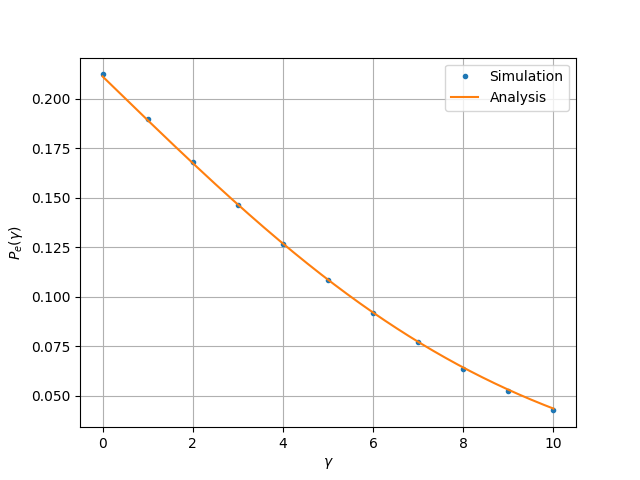
\includegraphics[width=\columnwidth]{figs/7_1.png}
	\caption{$P_e$ as a function of $\gamma$ (rectangular axes)}
	\label{fig:err-gamma}
\end{figure}
\begin{figure}[!htb]
	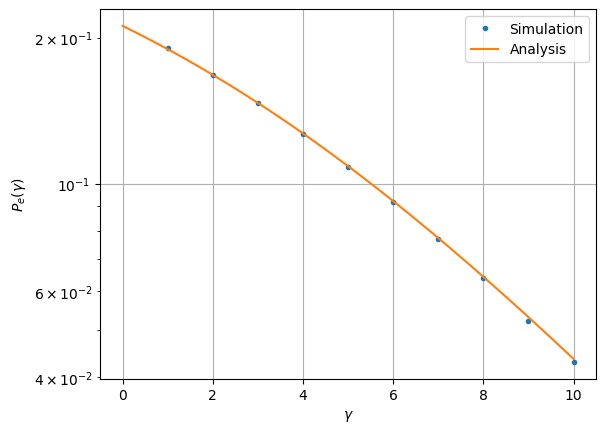
\includegraphics[width=\columnwidth]{figs/7_1_semilogy.png}
	\caption{$P_e$ as a function of $\gamma$ (semilog-y axes)}
	\label{fig:err-gamma-semilog}
\end{figure}
\item Assuming that $N$ is a constant, find an expression for $P_e$. Call this $P_e(N)$.

\solution
We rewrite the previous expression for $P_e$ as
\begin{align}
	P_e(N) &= \pr{A < -N} = F_A(-N) \\
	&= 
	\begin{cases}
		1 - e^{-\frac{N^2}{\gamma}} & N \leq 0 \\
		0 & N > 0
	\end{cases}
\end{align}

\item For a function $g$,
	\begin{align}
		E\sbrak{g(X)} = \int_{-\infty}^{\infty}g(x)p_X(x)dx
	\end{align}
Find $P_e = E\sbrak{P_e(N)}$.

\solution
We write,
		\begin{align}
			P_e &= \int_{0}^{\infty}F_A(x)f_N(x)dx \\
			&= \int_{0}^{\infty}(1 - e^{-\frac{x^2}{\gamma}})\frac{1}{\sqrt{2\pi}}e^{-\frac{x^2}{2}}dx \\
			&= \frac{1}{2} - \frac{1}{\sqrt{2\pi}}\int_{0}^{\infty}\exp{\brak{-\frac{x^2}{\frac{2\gamma}{\gamma + 2}}}}dx \\
			&= \frac{1}{2}\brak{1 - \sqrt{\frac{\gamma}{\gamma + 2}}}
			\label{eq:exp-err-ral}
		\end{align}
where $f_N$ denotes the standard normal distribution. 

\item Plot $P_e$ in problems 7.1 and 7.3 on the same graph wrt $\gamma$. Comment.

\solution
This has been done in Figure \eqref{fig:err-gamma} using the result \eqref{eq:exp-err-ral}. We observe that $P_{e|0} = E\sbrak{P_e(N)}$ i.e., the error rate is independent of the noise.
\end{enumerate}

\section{Two Dimensions}
\noindent Let 
\begin{align}
	\vec{y} = A\vec{x} + \vec{n}
\end{align}
where 
\begin{align}
	\vec{x} \in \brak{\vec{s}_0, \vec{s}_1}, \vec{s}_0 = \myvec{1 \\ 0}, \vec{s}_1 = \myvec{0 \\ 1} \\
	\vec{n} = \myvec{n_1 \\ n_2}, n_1, n_2 \sim \gauss{0}{1}
\end{align}
\begin{enumerate}[label=\thesection.\arabic*
,ref=\thesection.\theenumi]
\item Plot $\vec{y}|\vec{s_0}$ and $\vec{y}|\vec{s_1}$ on the same graph using a scatter plot.

\solution
The samples are generated in the C file in Question 1.1 as the files data/ber\_2D.dat and data/gau\_2D.dat. The generated random samples are then plotted taking $A = 5$dB in the Python code
\begin{lstlisting}
$ wget https://raw.githubusercontent.com/goats-9/ai1110-assignments/master/manual/codes/8_1.py
\end{lstlisting}
and the plot can be generated by running the code using
\begin{lstlisting}
$ python3 8_1.pyhow to add express sessions to login
\end{lstlisting}
\begin{figure}
	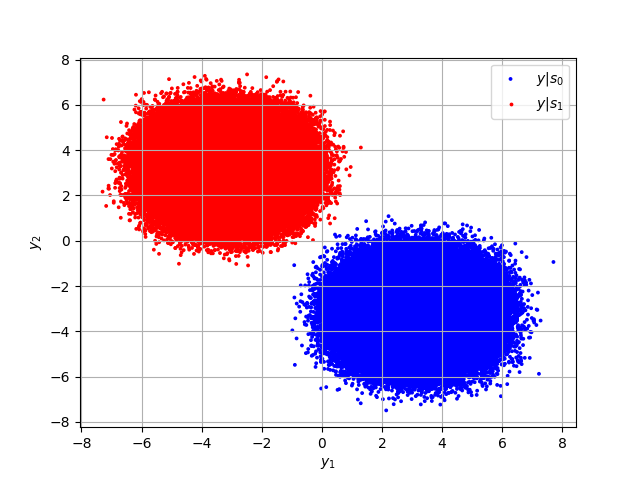
\includegraphics[width=\columnwidth]{figs/8_1.png}
	\caption{Scatterplot of $\vec{y}$, ($A = 5$dB)}
	\label{eq:y-scat-2D}
\end{figure}

\item For the above problem, find a decision rule for detecting the symbols $\vec{s}_0$ and $\vec{s}_1$.

\solution
The decision rule is 
\begin{align}
	\hat{\vec{x}} = 
	\begin{cases}
		\vec{s}_0 & y_1 > y_2 \\
		\vec{s}_1 & y_1 < y_2
	\end{cases}
\end{align}
where $\vec{y} = \myvec{y_1 \\ y_2}$
\item Plot 
	\begin{align}
		P_e = \pr{\hat{\vec{x}} = \vec{s}_1 | \vec{x} = \vec{s}_0}
	\end{align}
with respect to the SNR from 0 to 10 dB.

\solution
Download the Python codes
\begin{lstlisting}
$ wget https://raw.githubusercontent.com/goats-9/ai1110-assignments/master/manual/codes/8_3.py
$ wget https://raw.githubusercontent.com/goats-9/ai1110-assignments/master/manual/codes/8_3_semilogy.py
\end{lstlisting}
and run them with
\begin{lstlisting}
$ python3 8_3.py
$ python3 8_3_semilogy.py
\end{lstlisting}

\begin{figure}[!htb]
	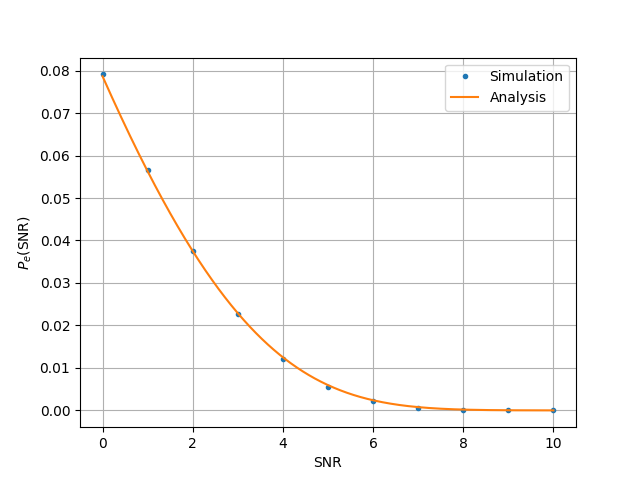
\includegraphics[width=\columnwidth]{figs/8_3.png}
	\caption{$P_e$ as a function of SNR (rectangular axes)}
	\label{fig:p-e-rect}
\end{figure}

\begin{figure}[!htb]
	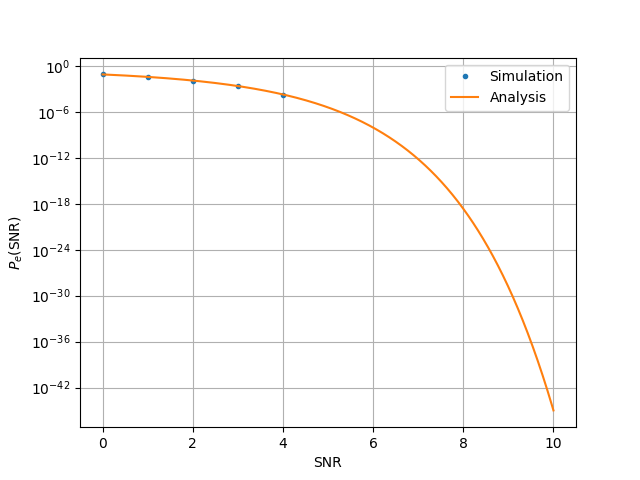
\includegraphics[width=\columnwidth]{figs/8_3_semilogy.png}
	\caption{$P_e$ as a function of SNR (semilog-y axes)}
	\label{fig:p-e-semilog}
\end{figure}

\item Obtain an expression for $P_e$. Verify this by comparing the theory and simulation plots on the same graph.

\solution
We have, 
\begin{align}
	P_e &= \pr{\hat{\vec{x}} = \vec{s}_1 | \vec{x} = \vec{s}_0} \\
		&= \pr{y_1 < y_2 | \vec{x} = \vec{s}_0} \\
		&= \pr{A + n_1 < -A + n_2} \\
		&= \pr{n_2 - n_1 > 2A} \\
		&= \pr{N > 2A} = \qfunc{\sqrt{2}A}
		\label{eq:p-e-2D}
\end{align}
where $N \define n_2 - n_1 \sim \gauss{0}{2}$ and $\textrm{SNR} = \frac{E\sbrak{A^2}}{\sigma_N^2}$.
\end{enumerate}
\end{document}
